\documentclass[11pt,a4paper]{article}

% pdfLaTeX input and font settings
\usepackage[utf8]{inputenc}
\usepackage[T1]{fontenc}

\usepackage[english,ngerman]{babel}                 % German and English word separation settings
\newcommand{\gqq}[1]{\glqq #1\grqq{}}               % Own command for german quotes
\usepackage{graphicx}                               % Include graphics/images
\usepackage{float}
\usepackage{multirow}                               % Row spanning over multiple rows
\usepackage{subcaption}                             % Used for 2 images side-by-side
\usepackage{tabularx}                               % for 'tabularx' environment
\usepackage[printonlyused,withpage]{acronym}        % Abkürzungsverzeichnis, https://de.wikibooks.org/wiki/LaTeX-W%C3%B6rterbuch:_Abk%C3%BCrzungsverzeichnis
\usepackage[bookmarks,                 % Creates bookmarks
            bookmarksnumbered=true,    % Numbers in PDF bookmarks
            bookmarksopen=true,        % Don't show bookmaks when opened
            hyperindex=true,           % Numbers in index are links
            pdfpagelabels=true,        % Set PDF page labels
            pdfa]{hyperref}                         % Klickable Links and ToC entries (should be last package !!!)

\hypersetup{
    pdfauthor    = {Thomas Gnaedig, Etienne Gramlich, Tim Hardenacke, Merle Wolff},
    pdftitle     = {DeepRain},
    pdfsubject   = {Deep Learning},
    pdfkeywords  = {Deep Learning,rain},
    pdflang      = {de},         % Set language of document to German
    pdfstartview = {FitH},       % Fit the document to screen horizontally (page width)
    pdfview      = {FitH},       % Fit the document to screen horizontally (page width)
    colorlinks   = {true},       % Use color for links
    linkcolor    = {black},      % Links in black (text color)
    urlcolor     = {black},      % URLs in black (text color)
    citecolor    = {black},      % Citations in black (text color)
    filecolor    = {black},      % File links in black (text color)
}

\title{DeepRain}
\author{Thomas Gnaedig, Etienne Gramlich, Tim Hardenacke, Merle Wolf}

\begin{document}
\maketitle
\tableofcontents

\begin{acronym}[Bash] % Hier steht die längste Abkürzung, damit die Breite stimmt
 \acro{DL}{Deep Learning}
 \acro{Bash}{Bourne-again shell}
 \acro{VM}{Virtuelle Maschine}
\end{acronym}

% Abstract
\begin{abstract}
Die Niederschlagvorhersage geschieht oft mit Modellen aus der Meteorologie, die auf physikalischen Gesetzen passieren. Unser Ziel war es zu bestimmen, ob der Niederschlag mit Methoden des Maschinellen Lernens vorhergesagt werden kann.

Dazu vergleichen wir verschiedene Typen von neuronalen Netzen und trainieren sie mit Daten des Deutschen Wetterdienstes und präsentieren die Ergebnisse und Genauigkeit für die Stadt Konstanz und ganz Deutschland.~\cite{DBLP:journals/corr/RonnebergerFB15}
\end{abstract}

%Einleitung zu DeepLearning
\section{Abstract}
Das Teamprojekt DeepRain bestehend aus fünf Studierenden der Masterstudiengänge MSI und BIT startete im Wintersemester 18/19 an der HTWG Konstanz. Das Ziel Projekts ist, innerhalb eines Jahres einen lauffähigen Algorithmus auf Github (thgnaedi/DeepRain) zur Verfügung zu stellen. Dieser soll mit Hilfe von Deep Learning in der Lage sein das Wetter, bzw. den Niederschlag, in Konstanz über den Zeitraum von einer Stunde vorherzusagen. Das einjährige Projekt wird von Prof. Oliver Duerr betreut. 
Eine möglichst genaue Wettervorhersage hat viele offensichtliche Vorteile. Beginnend mit dem täglichen Verlassen des Hauses und der Entscheidung; mit oder ohne den Regenschirm? Vermutlich treffen die meisten diese Entscheidung basierend auf der Wettervorhersage und vertrauen darauf, dass diese auch korrekt ist.
Vorhersagen mit Deep Learning-Unterstützung finden auch eine sehr wichtige Verwendung in der Katastrophenvorhersage und dem Katastrophenmanagement (vgl. \cite[S. 763]{Hanif.2019}). Eine weitere wichtige Rolle spielt es bei der Energieversorgung, beispielsweise bei der Planung der Auslastung von Solar-Panels (vgl. \cite[S. 2]{AndreGensleret.al..}). Die eigentliche Wettervorhersage wird jedoch bisher noch nicht mit Deep Learning-Techniken generiert, dies ist erst ab diesem Jahr bei einigen Anbietern angedacht (vgl. \cite{ChristophFrohlich.2019}. 
\begin{figure}[ht]
\centering
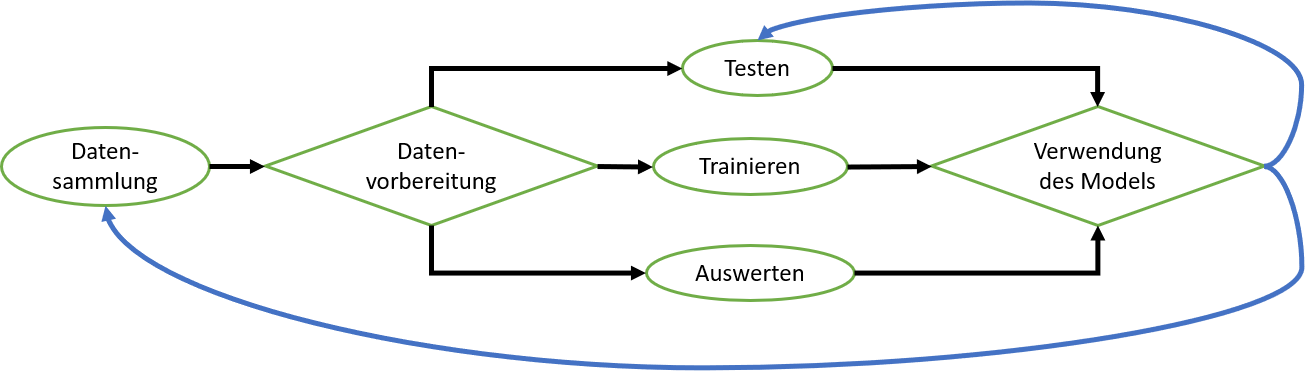
\includegraphics[width=\linewidth]{pics/Deep_learning_prozess}
\caption{Wichtige Schritte im Prozess des DeepRain-Projekts, eigene Darstellung}
\label{fig:deepLearningProcess}
\end{figure}
Im Rahmen des Teamprojekts stand zu Beginn ein einarbeiten in die Prozesse des Maschine-Learnings an, sowie den Stand der Technik zu recherchieren. Daraufhin stand die Datenbeschaffung im Vordergrund und die Qualitätsbewertung der vorhandenen Daten. Im späteren Verlauf des Projekts ging es dann an die Entwicklung des Algorithmus. Der Ablauf dieser Arbeit lehnt sich an diesen, auch in Abbildung~\ref{fig:deepLearningProcess} dargestellten, Prozess an. 

\subsection{Deep Learning}
Deep Learning basiert auf der Optimierung von künstlichen neuronalen Netzen (KNN) und ist eine Weiterentwicklung des Maschine Learning (vgl. \cite[S. 1]{Georgevici.2019}). Ziel von neuronalen Netzen ist es, eine ähnliche Lösungsweise zu ermöglichen, wie im menschlichen Gehirn. Kern ist hier das “Lernen” und das Lösen von Problemen. Neuronale Netze haben sich vor allem wegen ihrer Fähigkeit der Verarbeitung von ständig wachsenden Datenmengen und -komplexität etabliert (vgl. \cite[S. 373]{Welsch.2018}). In einem künstlichen neuronalen Netzwerk müssen im Vorhinein keine Vermutungen über Zusammenhänge festgelegt werden, denn diese werden während des Lernprozesses vom Netz ermittelt (vgl. \cite[S. 581]{Backhaus.2018b}). Ein Neuronales Netz ist 
so aufgebaut, dass es einen bekannten Input gibt, welcher durch einen sogenannten Hidden-Layer läuft. Der Hidden-Layer besteht aus Neuronen in denen das Lernen stattfindet und schließlich ein Output generiert wird. Dabei können einige Variablen, die den Output beeinflussen, festgelegt werden. 
Die Neuronen modifizieren dabei die Daten und leiten diese anschließend weiter (vgl. \cite[S. 373]{Welsch.2018}). Es kann sich auch zwischen einer biologischen oder einer technischen Simulation von Neuronen entschieden werden (vgl. \cite{https:www.facebook.comspektrumverlag.04.12.2014}). Die technische Simulation wird zur Datenverarbeitung und Mustererkennung meist bevorzugt (vgl. \cite{https:www.facebook.comspektrumverlag.04.12.2014}). Dieser Zusammenhang wird in Abbildung~\ref{fig:NeuralVsDeepNeural} dargestellt. 
In dieser Abbildung wird auch ersichtlich, wodurch sich ein Deep Neural Network von einem neuralen Netz unterscheidet. Hier wird gleich mit mehreren Hidden-Layers, die hintereinander liegen, gearbeitet. Die Verwendung mehrerer Hidden-Layers führt dabei laut (\cite[S. 581]{Backhaus.2018b}) zu erfahrungsgemäß korrekteren Lernergebnissen. Das „Lernen“ hängt dann vom Grad der Aktivierung der einzelnen Neuronen ab. Dieser wird durch die bisherigen Ergebnisse durch eine ermittelte Gewichtung einzelner Neuronen bestimmt. Diese Gewichtung wird im Verlauf des Lernens im Netz im besten Fall immer weiter optimiert (vgl. \cite[S. 586]{Backhaus.2018b}).
\begin{figure}[ht]
\centering
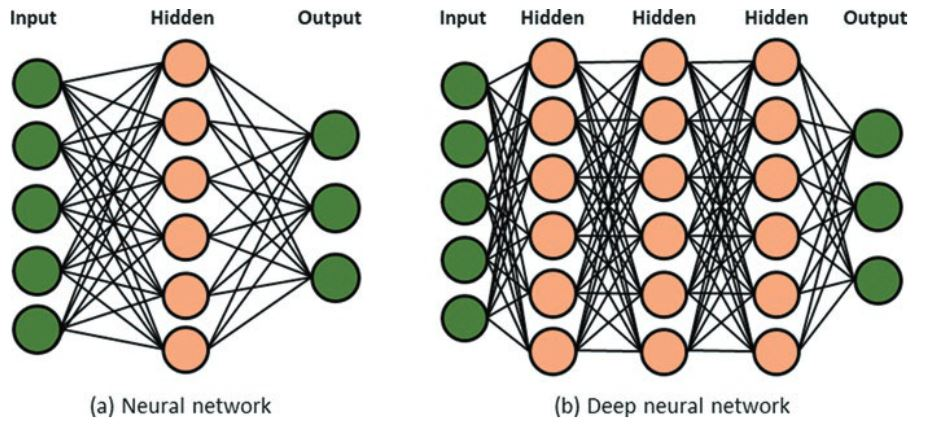
\includegraphics[width=\linewidth]{pics/ANN_for_deep_learning_P35}
\caption{Unterscheidung Neurales Netzwerk und Deep-neurales Netzwerk, Quelle: ANN for deep learning (Akerkar 2019, S. 35)}
\label{fig:NeuralVsDeepNeural}
\end{figure}
In unserem Projekt soll mithilfe von neuronalen Netzen, das Lernen aus bisherigen Wetterdaten ermöglicht werden, sodass eine möglichst korrekte Wettervorhersage der kommenden Stunde generiert wird.

\subsection{State-of-the-art Wettervorhersage mit Deep Learning}
Obwohl für Deep Learning, Machine-Learning, sowie Neuro- und Lingual-Programming einiges an Literatur zu finden ist, steht die Nutzung zur Wettervorhersage noch am Anfang (vgl. \cite{ChristophFrohlich.2019}). So gibt es auf der Plattform GitHub zum aktuellen Stand (August 2019) gerade einmal eine Handvoll Repositories zum Thema Wettervorhersage mit Deep Learning. Verfahren werden verbessert, die Lernverfahren den Menschlichen Lernen immer ähnlicher, die Entwicklung ist stetig steigend und wie bereits erwähnt sind noch viele Bereiche wie u.a. die Wettervorhersage  ergründbar (\cite[S. 103]{Wick.2017}). Im Bereich der Wettervorhersage bietet sich, in Anlehnung an Abbildung 3, in den meisten Fällen das Supervised Learning an, da eine möglichst genaue Vorhersage erreicht werden soll. Aber auch das  nicht-überwachte Lernen kann interessante Schlüsse zulassen, um eventuell unbekannte Muster zu finden (vgl. \cite[S. 371]{Welsch.2018}). 


\section{Daten}
Dieses Kapitel geht darauf ein, woher wir die Daten für das Training des Netzes beschaffen und wie wir diese vor-bearbeiten.

\subsection{Quelle}
Die verwendeten Daten stammen vom Deutschen Wetterdienst (ab jetzt DWD) und sind Radardaten von deren Radarstationen. Die Daten der Messstationen bilden Kreise um die jeweiligen Stationen und bedecken noch einen kleinen Bereich um Deutschland; die Daten geben die Stärke des Niederschlags an. Die Radar-Messungen liegen in einer Auflösung von einer Stunde und 5 Minuten vor, wir verwenden letztere. Z.zt. liegen die Daten vom Januar 2001 bis Januar 2018 vor (jeweils inklusive). Für unsere Zwecke verwenden wir die 18 kompletten Jahre 2001 bis 2017.\footnote{\url{https://opendata.dwd.de/climate\_environment/CDC/grids\_germany/5\_minutes/radolan/reproc/2017\_002/bin/}}

\subsubsection{Crawler}
Da die Daten in monatsweise in geschachtelten Archiven gepackt sind, haben wir einen Crawler geschrieben, der die Daten zuerst herunterlädt und auspackt. Mit den Kommandozeilenoptionen\footnote{\url{https://github.com/thgnaedi/DeepRain/tree/master/DWD_Crawler}} kann gesteuert werden, ob die stündlichen oder minütlichen Daten heruntergeladen werden und wohin die Binärdateien entpackt werden sollen. Wir empfehlen, die Binärdaten auf eine Btrfs\footnote{\url{https://en.wikipedia.org/wiki/Btrfs}}-formatierte Partition zu entpacken, da die Daten (wegen häufig auftretender Nullen bzw. kein Regen) leicht komprimierbar sind und die minütlichen Daten sonst mehr als ein Terabyte belegen würden.

\subsection{Preprocessing}
Um das Binärformat des DWD einzulesen, benötigt man die Python-Bibliothek \gqq{Wradlib}, die man über den Package-Manager von Anaconda installieren kann. Dann kann man die Datensätze als Deutschlandkarte mit einer Auflösung von 1100x900 Pixeln rastern.

Das Preprocessing geschieht in zwei Durchläufen: Zuerst wird das Maximum des Niederschlags bestimmt, das Minimum wird als 0 (kein Regen) angenommen. Danach werden die Werte auf einen Bereich gespreizt.

Beim zweiten Durchgang werden die Daten mithilfe des globalen Maximalwertes auf einen Wertebereich zwischen 0 und 255 umgerechnet, damit die Datensätze in einem Bildformat mit einer Bittiefe von 8 Bit gespeichert zur weiteren Verarbeitung werden können. Wir haben uns für das PNG-Format entschieden, weil es verlustfrei komprimiert und von platt­form­über­grei­fenden Bibliotheken gelesen und geschrieben werden kann.
Vor dem Speichern werden die Werte mit dem Faktor 4 multipliziert um Werte über 255 auf den Maximalwert abzuschneiden. Dadurch verwerfen wir Ausreißer und das Training funktioniert besser. Der Faktor 4 wurde empirisch bestimmt, weil das Berechnen eines Histogramms über alle 18 Jahre zu aufwendig gewesen wäre.

\subsection{Herausforderungen in diesem Kapitel}
Die größte Herausforderung in diesem Kapitel war zweifelsfrei die große Datenmenge, die wir verarbeitet haben. Die Rohdaten der 18 Jahre in 5-Minuten-Auflösung hätte unseren zugewiesenen Speicher gesprengt. Mit Btrfs, das die Dateien on-the-fly komprimiert und de-dupliziert, passten die Daten doch auf unsere Festplatte. Auch mussten wir eventuelle Ausreißer empirisch entfernen, weil das Berechnen des Histogramm über so viele Daten zu aufwendig wäre.

Darüber hinaus lagen die Archive des DWD im Tar-Format vor, das keine Checksumme anbietet und somit erst beim Entpacken bemerkt werden kann, dass beim Download einer Datei ein Fehler auftrat. Bei den großen Tar-Archiven des DWD ist leider mehrmals ein Download-Fehler aufgetreten, der sehr spät auffiel.


% Datenaufbereitung
\section{Daten-Aufbereitung}

\subsection{RADOLAN-Daten}

Die Daten des DWD werden über das Routineverfahren RADOLAN (Radar-Online-Aneichung) erfasst, dass durch eine Kombination von Niederschlagstationen und Wetterradaren hochauflösende Niederschlagsdaten produziert. 

Die Open-Source Bibliothek wradlib \footnote{\url{https://docs.wradlib.org/en/stable/index.html}} stellt für diese RADOLAN-Daten eine Stereographische Projektion zur Verfügung. Dies bedeutet das die Erdkugel zu einem Koordinatensystem aufgespannt wird, dessen Ursprung im Nordpol liegt. Siehe Abbildung  \ref{rz}.

\begin{figure}[H]
	\centering
	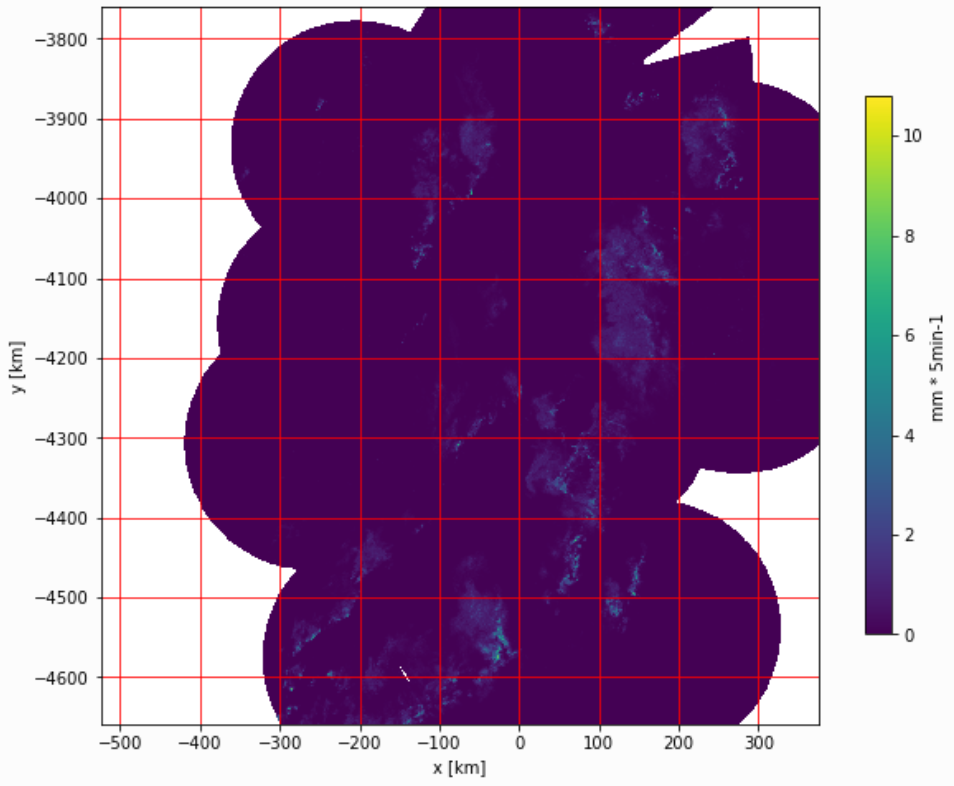
\includegraphics[width=0.8\textwidth]{pics/RZ_product.PNG}
	\caption{Ausschnitt Deutschlands im Koordinatensystem}
	\label{rz}
\end{figure}

Der resultierende Ausschnitt für Deutschland kann mit Hilfe von wradlib als 1100 * 900 Array ausgelesen werten, dessen Werte einer 1 Kilometer Grid-Box entsprechen.

\subsection{Location Konstanz}
Um für Konstanz und Umgebung sinnvolle Vorhersagen treffen zu können, muss der Standort von Konstanz auf den Daten markiert werden. Dazu müssen die geographischen Koordinaten von Konstanz in X- und Y-Koordinaten des Koordinatensystems umgewandelt werden.

\begin{table}[H]
\centering
\begin{tabularx}{8cm}{X|X}
\multicolumn{2}{c}{Geographische Koordinaten}\\
\textbf{Latitude} & \textbf{Longditude}\\\hline
47.66033          & 9.17582\\
\end{tabularx} 	
\end{table}

\begin{table}[H]
\centering
\begin{tabularx}{8cm}{X|X}
\multicolumn{2}{c}{XY - Koordinaten}\\
\textbf{X-Koordinate} & \textbf{Y-Koordinate}\\\hline
-4602.6447            & -66.4622\\
\end{tabularx} 	
\end{table}

Die umgewandelten XY-Koordinaten müssen nun innerhalb des Arrays gefunden werden. Dazu wurde über den Array iteriert und die Werte mit den errechneten Werten verglichen. Anschließend muss die Location auf der Karte markiert und dargestellt werden (siehe Abbildung~\ref{fig:location}).

\begin{figure}[H]
	\centering
	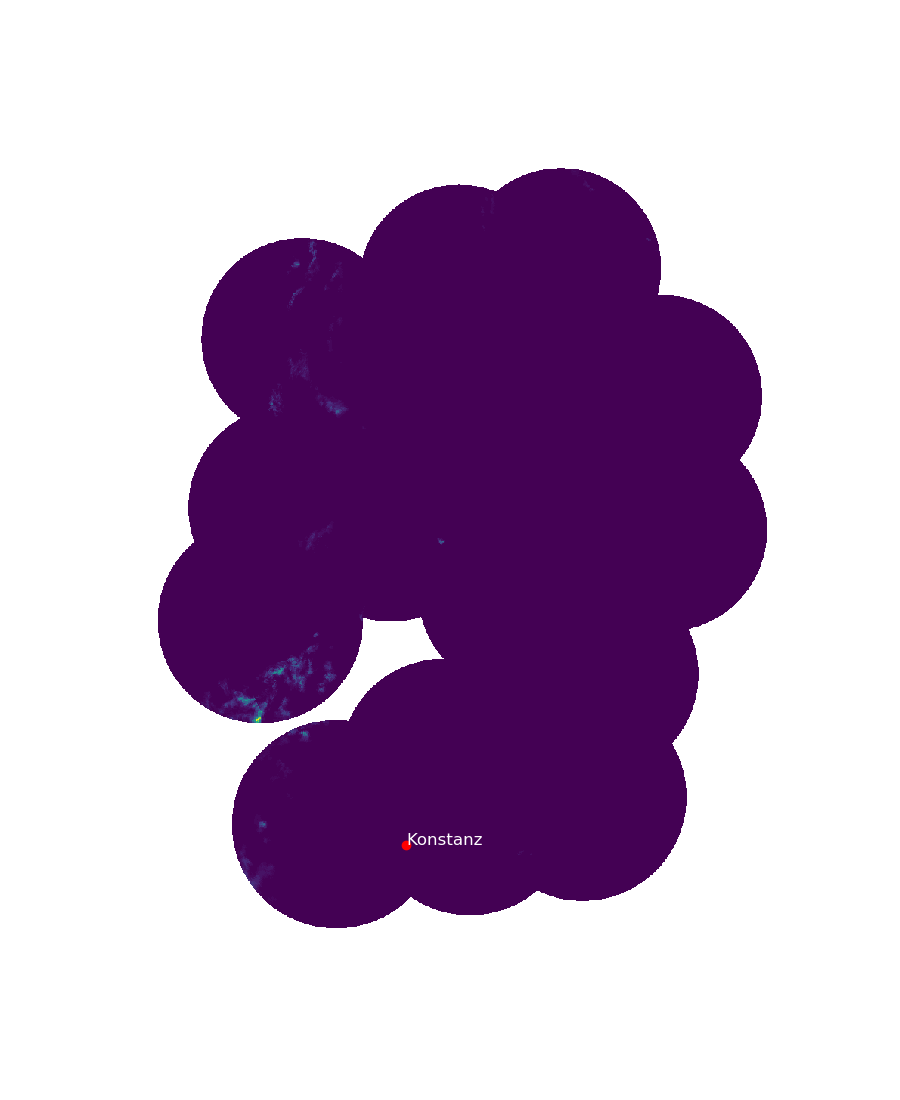
\includegraphics[width=0.8\textwidth]{pics/Location.png}
	\caption{Location von Konstanz im Ausschnitt Deutschland}
	\label{fig:location}
\end{figure}

\subsection{Herausforderungen} 
Änderungen der Auflösung des Formats anpassen, richtige Datenquelle in wradlib finden. XY-Koordinaten innerhalb des Arrays finden und darstellen.

% Datenanalyse
\section{Datenanalyse}
Es wurden im Projekt unterschiedliche Daten auf ihre Quantität, Qualität und Verwendbarkeit untersucht. In diesem Schritt betrifft die Datenqualität erstmal die äußerlichen Merkmale, die tatsächliche Ähnlichkeit und der Vergleich von Regendaten folgt in einem späteren Kapitel. 
Für das Projekt werden zum einen die tatsächlichen Niederschlagsdaten in Konstanz zum späteren Vergleich benötigt, zum anderen Radardaten, beides möglichst in ein bis zehnminütlicher Auflösung und möglichst von aktuell bis einige Jahre in die Vergangenheit reichend. 
Wetterradardaten werden von öffentlichen und privaten Anbietern erhoben und sind in unterschiedlichen Qualitäten und unterschiedlicher Datenmenge verfügbar. Der Email-Verkehr mit Meteogroup, einem privaten Wetterdienstleiter zeigte, dass die Daten der Wetterstationen Konstanz Südkurier und Konstanz Dettingen von uns nicht verwendet werden konnten. Die Daten von Windy sind zwar öffentlich zugänglich, jedoch nicht dowloadbar, welches eine Voraussetzung für verwendete Daten ist. Die Daten die Anbieters Kachelmann sind bis ins Jahr 2015 online verfügbar jedoch müssten hier die Nutzungsrechte eindeutig geklärt werden. 
Die umfangreichsten Radardaten werden von der Deutschen Wetterstation zur Verfügung gestellt, daher wurde sich im Team für die Verwendung dieser Daten entschieden. 

\subsection{Verifizierung der Daten mit statista und Wetterkontor}
In den Daten des DWD hat die Konstanzer Wetterstation die ID: 02712. Aus dem Zip-File mit der enthaltenen Textdatei können somit die nun aufgezeigten Daten für die Untersuchung entnommen werden. Zu den wichtigsten Informationen gehören hier das Qualitätsniveau der Daten (zwischen 1 und 16) als QN, das Messdatum im Format YYYYMMDDHHMM, die Niederschlagshöhe und den Niederschlagindikator. Die Aktuellen Daten wurden mit einem Python-Script eingelesen und ein paar kleine Statistiken zum Validieren der Daten vorgenommen. Zum Vergleich wurden hierfür die monatlichen Niederschlagsangaben von Statista.com und Wetterkontor.com genommen, allerdings bezogen die sich auf ganz Deutschland.
\begin{table}[ht]
\centering
\begin{tabular}{ll|l|ll}
\textbf{Monat} & \textbf{ref. $l/m^2$} & \textbf{Messung} & \textbf{Fehler (abs.)} & \textbf{Fehler (rel.)}\\\hline
Januar    & 40,1  & 37,39  & -2,71  & 6,76\%\\
Februar   & 34,5  & 37,02  & 2,52   & 7,30\%\\
März      & 40,2  & 40,3   & 0,1    & 0,25\%\\
April     & 132,4 & 132,25 & -0,15  & 0,11\%\\
Mai       & 56,4  & 52,58  & -3,82  & 6,77\%\\
Juni      & 95    & 69,55  & -25,45 & 26,79\%\\
Juli      & 168,9 & 171,38 & 2,48   & 1,47\%\\
August    & 155,7 & 148,42 & -7,28  & 4,68\%\\
September & 65    & 55,23  & -9,77  & 15,03\%\\
Oktober   & 36,3  & 36,93  & 0,63   & 1,74\%\\
November  & 76,8  & 78,49  & 3,69   & 4,93\%\\
Dezember  & 79,5  & 78,52  & -0,98  & 1,23\%\\
\end{tabular}
\caption{Auswertung des absoluten und relativen Fehlers zwischen den Regendaten verschiedener Quellen}
\label{tab:Auswertung}
\end{table}

Die Historischen Daten des DWDs sind auch Monatlich als Textdatei gespeichert. Für den Vergleich wurde das Jahr 2018 betrachtet. In den historischen Daten fallen neue Spalten im Header auf, diese sind aber \gqq{ungenutzt} bzw. über alle (geprüft auf Jahr 2017) Einträge identisch. Diese sind: QN, RTH\_01 und RWH\_01. Die Messwerte wurden wie auch zuvor monatsweise zusammenaddiert das Ergebnis des Vergleichs ist in Tabelle~\ref{tab:Auswertung} zu sehen. 
Auffällig ist, dass einige Messwerte sehr gut übereinstimmen. So ist der Niederschlag in den Monaten März und April fast gleich in der referenzierten Messung und der Messung des DWDs. In anderen Monaten wie im Juni ist der relative Fehler mit 26.79\% sehr hoch. Das könnte an gemessenen Extremwerten in den Daten des DWDs liegen, die in der Größenordnung in den Messungen der anderen Anbieter nicht auftauchen.
Die hierzu verwendeten Skripte und Quellen sind auf github wiederzufinden \footnote{\url{https://github.com/thgnaedi/DeepRain/tree/master/WetterStation_KN}}.  

\subsection{Korrelation der Radardaten mit den Regenmessungen}

In diesem Schritt sollte geprüft werden, wie hoch die gemessenen Radardaten mit den Niederschlagsdaten korrelieren. Im optimalen Fall sollten alleine auf Grundlage dieser Analyse Rückschlüsse auf die Lage von Konstanz auf dem Radarbildern durch eine besonders hohe Korrelation der Daten möglich sein. Als Monat für die Untersuchung wurde der Juni 2016 gewählt, da es sich um einen sehr Regenreichen Monat gehandelt hat.
Einen wichtigen Anteil an der Korrelationsanalyse hat die Datenaufbereitung in Anspruch genommen. Um einen Vergleich der Niederschlagsdaten mit den Radardaten zu ermöglichen ist es erforderlich, dass die Daten jeweils für dieselben Zeitabstände verfügbar sind. Da die Regenmessungen in minütiger Auflösung vorliegen, wurden sie mit Hilfe zweier Python-Skripte auf eine Datei mit 5-minütiger und eine mit stündlicher Auflösung angepasst. Nun wurde ein Notebook geschrieben, dass die Pixelwerte der Punkte um Konstanz also den Pixelwert 842.406 herum einliest und mit dem Zeitpunkt der Messung und dem tatsächlich gemessenen Niederschlag zu diesem Zeitpunkt in einer Numpy-Matrix speichert. Hier musste eine Einschränkung in Kauf genommen werden, da das einlesen jedes einzelnen Pixels bei 900 x 1100 Pixeln nicht möglich war und daher circa ein Umkreis von 20 Pixeln um Konstanz herum ausgewählt wurde. Bei der ersten Analyse wurde mit 156.377 ein falscher Pixel verwendet, was auf Unklarheiten bei der Achsenbestimmung zurückzuführen war. Die erstellte Numpy-Matrix wurde dann noch auf fehlende Werte untersucht, dieser Anteil hat sich als verschwindend gering herausgestellt, das heißt, dass die Daten bis auf ganz wenige Ausreißer vollständig sind. 
\begin{figure}[ht]
\centering
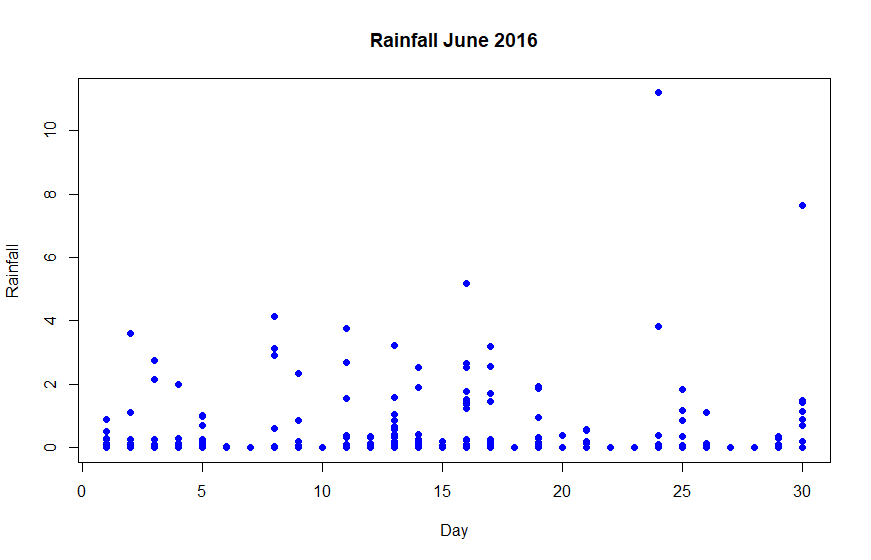
\includegraphics[width=\linewidth]{pics/plot_rainfall_day}
\caption{Regenfallmengen im Juni 2016 nach Tag}
\label{fig:Rainfall}
\end{figure}
Für die Analyse der Daten wurde dann ein R-Skript geschrieben. In diesem wurden die Datuminformationen extrahiert, sodass eine Einteilung in Jahr, Monat, Tag, Stunde und Minute der Datensätze möglich wurde. Dann wurden die die Regenmengen der gemessenen Niederschlagswerte je Tag dargestellt. Hier zeigte sich eine recht gleichmäßige Verteilung der Regenwerte mit einigen gut identifizierbaren Ausreißern z.B. am den 24. Juni mit über zehn Liter pro Quadratmeter, siehe \ref{fig:Rainfall}. Bei der Werteverteilung der Pixel aus den Radarbildern fällt auf, dass es sehr viele null-Werte und am zweitmeisten den Wert 80 gibt. Werte, die dazwischen existieren sind „10“, „20“, und „40“.  Bezüglich der Niederschlagsdaten könnte hier auch das eher niedrige Qualitätsniveau der Stufe 3 Einfluss gehabt haben.
Leider konnte zwischen den beiden Datentypen keine Korrelation festgestellt werden. Hierfür kommt eine Reihe von möglichen Gründen in Frage. Da die eigene Betrachtung der Daten, also der händische Abgleich von Zeiten mit Starken Regen in beiden Datengruppen nahelegt, dass die Daten tatsächlich nicht korrelieren kommt in Frage, dass die gemessenen Daten der Wetterstation Konstanz Fehlmessungen beinhalten. 

% Netzwerke
\section{Netzwerkarchitekturen}
%erster Kontakt MNIST wie viel Trefferrate mit einfacher architektur
Für den ersten Kontakt mit einem Neuronalen Netz befassten wir uns mit dem MNIST Datensatz. Hierbei geht es um eine Klassifizierung von Handschriftlichen Zahlen in die zugehörigen zehn Klassen. Um Rechenzeit zu sparen, da uns Anfangs noch keine GPU zur Verfügung stand, haben wir das Netz sehr klein gehalten. Das Netz für welches wir uns entschieden haben, besteht aus einem Convolutional Layer mit 32 3x3 Kerneln, diese werden im späteren Kapitel \ref{kapitelCNN} genauer erläutert. Anschließend folgt ein 2x2 MaxPooling Layer, auch darauf gehen wir später noch ein. Um die Klassifikation vornehmen zu können, wird anschließen ein Flatten Layer eingebunden und ein Fully-Connected Layer mit 128 output Neuronen. Diese 128 Features werden dann über ein weiteres Fully-Connected Layer auf die 10 Ausgabeklassen verrechnet. Als Aktivierungsfunktion dient ein softmax, welcher dafür sorgt, dass die summe aller ausgaben Eins ergibt. Somit können die Outputs als Wahrscheinlichkeiten gedeutet werden, die Wahrscheinlichste Klasse wird dann als Vorhersage verwendet.
Das hier erwähnte Fully-Connected Layer ist die einfachste Art eines Layers, es besteht aus mehreren Eingabeneuronen und einigen Ausgabeneuronen. Jedes Ausgabeneuron ist hierbei mit jedem Eingabeneuron verbunden. Um den Wert eines Ausgabeneurons zu berechnen wird dann einfach eine gewichtete Summe aller Eingaben berechnet. Die hierbei verwendeten Gewichte werden über die Fehlerfunktion gelernt.

%Aufgabenstellung bzw. Lösung
Für die kurzzeit Wettervorhersage entschieden wir uns für zwei grundlegende Aufgabenstellungen. Die erste Herangehensweise war das vorhersagen weiterer Radarbilder in der Zukunft. Die Architektur muss also mehrere zusammengehörende Radarbilder als Eingabe verarbeiten und als Ausgabe wieder ein oder mehrere Zeitschritte liefern. Für diese Aufgabenstellung eignet sich sowohl ein Klasisches CNN (Kaptel \ref{kapitelCNN}), als auch ein UNet(Kaptel \ref{kapitelUNet}). Um uns zwischen diesen Architekturen zu entscheiden nahmen wir einen kurzen Test vor, in welchem beide Architekturen mittels MSE einen Zeitschritt (5minuten) vorhersagen sollten.
\begin{figure}[h]
	\centering
	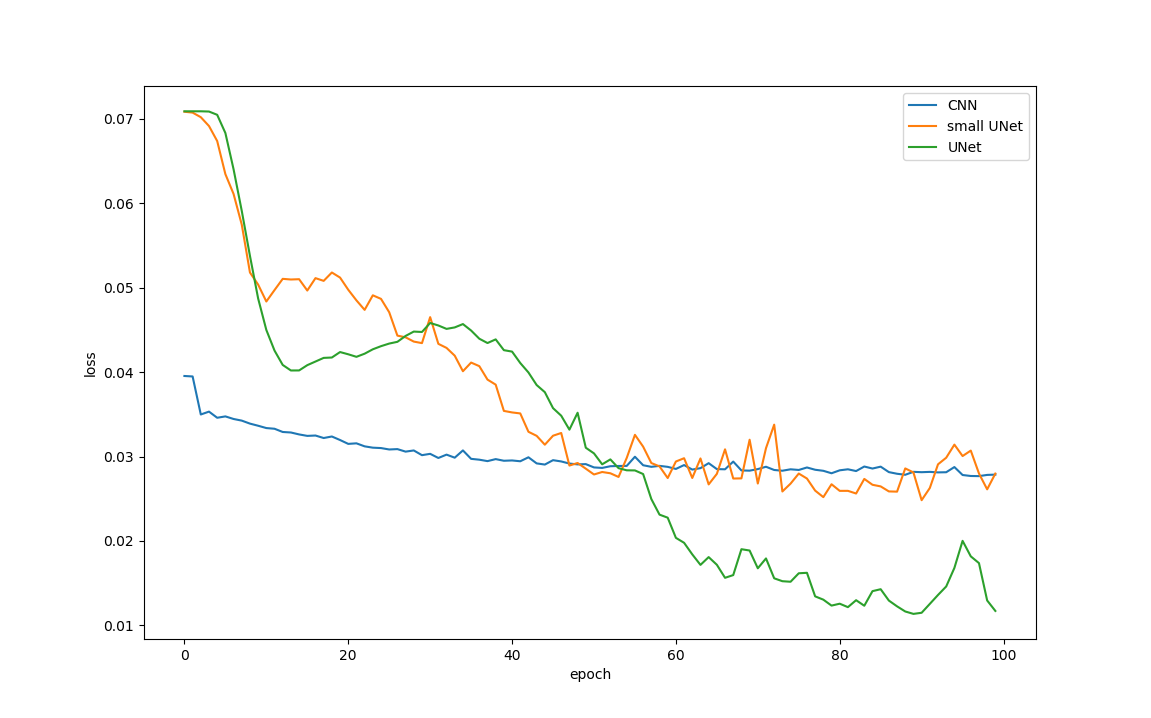
\includegraphics[width=\linewidth]{pics/Syntetische_Daten_CNN_UNet.png}
	\caption[Lernkurven verschiedener Architekturen auf Syntetische Daten]{Gezeigt ist die Lernkurve der Validierungsdaten auf 100 Epochen mit unterschiedlichen Netzarchitekturen. Die Verwendeten Trainingsdaten sind 1000 syntetische Bilder welche eine wandernde Regenfront Simulieren sollen. Das CNN ist etwa gleich gut wie das einfache UNet. Eine tiefere UNet Architektur (grün) erreicht eine noch bessere Performance. Die Architekturen sind in nachfolgenden Kapiteln genauer erläutert. }
	\label{imgCNNUNet}
\end{figure}

Die Abbildung \ref{imgCNNUNet} zeigt die Lernkurve der beiden Architekturen auf die Identische Problemstellung. Das UNet lernt in diesem Beispiel deutlich besser, weshalb die Vorhersage von Radarbildern in Zukunft mit einem UNet behandelt wird. Beide UNet Architekturen haben zu beginn eine deutlich schlechtere Vorhersage als das CNN, bereits nach 60 Epochen ist die einfache UNet Architektur gleich gut, während das grüne UNet die Performance sogar übertrifft und nach 100 Epochen die besten Ergebnisse liefert.
\newline
Die zweite Herangehensweise ist eine Klassifikation, hierbei geht es nicht darum das exakte Radarbild vorherzusagen, sondern einzuordnen, ob es Regnet oder nicht. Diese Aufgabe wurde als einfache Klassifikation für Konstanz, als auch als Pixelweise Klassifikation, für alle eingehenden Pixel durchgeführt. Für die Aufgabe der Klassifikation jedes Pixels wurde wieder ein UNet verwendet. Bei der Aufgabe der einfachen Klassifikation für Konstanz kamen beide Architekturen zum Einsatz.

\subsection{CNN}
\label{kapitelCNN}
Ein Convolutional Neural Networks im klassischen Sinne ist ein Netzwerk mit mehreren Convolutional-Layer, häufig in verbindung mit Pooling-Layer. Ein Convolutional-Layer besteht aus mehreren Filtern. Die Filter berechnen ein Output in abhängigkeit mehrerer Benachbarter 'Pixel' die größe der berücksichtigten Region hängt von der Filter- bzw. Kernelgröße ab.
Vorteile von Convolutional Layern sind zum einen, dass Nachbarschaften berücksichtigt werden, was gerade bei Bildern sehr sinnvoll ist, aber auch, dass der Speicherbedarf sehr gering ist, da nur eine kleine Anzahl an Gewichten für das Komplette Bild verwendet werden müssen.
Ein Pooling-Layer reduziert die Feature-Größe indem jeweils nur das stärkste Signal einer Region weitergegeben werden.

%MSE:
Für die Vorhersage der Radardaten haben wir uns für ein sehr einfaches CNN (Convolutional Neural Network) entschieden.
Als Eingabe erwartet es mehrere Zeitschritte um darauf eine Vorhersage zu treffen. Der input ist also dreidimensional wobei die dritte dimension die Zeitschritte und die anderen Dimensionen die Bildauflösung beschreiben. Die Eingabe wird durch sechzehn Convolution Kernel der Größe 5x5 verrechnet. Anschließend folgen zweiunddreißig weitere 5x5 Kernel. Anschließend ist ein optionales Dropout Layer eingebunden, welches nur zu Testzwecken verwendet wurde. Die Performance hatte sich dadurch aber nicht bemerkenswert verändert. Abschließend kommt ein Kernel, welcher die nun entstandenen Features zu einem Bild zusammenfasst. Hierzu wird ein 3x3 Kernel verwendet. Alle Layer sind mit einer ReLu als Aktivierungsfunktion ausgestattet.
Die Performance ist weniger gut, als ein UNet kann aber mit der sehr einfachen UNet Architektur mithalten. Zu sehen ist das in Abbildung \ref{imgCNNUNet} wo die Blaue Kurve dem Lernverhalten der hier beschriebenen CNN Architektur entspricht.

%Klassifikation:
Für Klassifikation des Konstanzpixels entschlossen wir uns dazu das CNN welches wir eingangs verwendet hatten um den MNIST Datensatz zu lernen wieder zu verwenden. Dieses Netz besteht lediglich aus zweiunddreißig 3x3 Kerneln mit ReLu aktivierungsfunktion. Anschließend folgt ein 2x2 MaxPooling und ein Flatten Layer. Die nun "Flachen" Daten werden durch ein FullyConnected Layer auf 30 Neuronen reduziert. Darauf folgt ein Dropout Layer mit 20\% welches Overfitting verhindern soll. Abschließend Folgt ein Layer das die Features auf drei ausgabe Neuronen verrechnet. Damit die Klassifizierung einfacher zu interpretieren ist, wird als aktivierungsfunktion ein SoftMax verwendet.

\subsection{UNet}
\label{kapitelUNet}
%was ist ein Unet?
Ein Unet ist eine spezielle Form eines CNN. Es hat seinen Namen durch die 'U-Förmige' Architektur, siehe Abbildung
ToDo: ref für UNet img.
Das Unet besteht aus mehreren Convolutional Layern, mit anschließendem Pooling. Hierdurch wird die Featuregröße immer weiter Reduziert. Ab einem bestimmten Punkt wird die Featuregröße wieder aufgeblasen, um schlussendlich am output die gleiche Größe wie am Input zu besitzen. Beim 'aufblasen' kommt ein Upsampling Layer zum Einsatz. Da allerdings beim vergrößern der Features nicht alle Informationen wiederhergestellt werden können gibt es auch noch horizontale Verbindungen, durch welche zuvor erstellte Features später weiterverwendet werden können.
Diese Architektur ist sehr ähnlich zu einem Autoencoder und wurde erstmals für biomedizinische Zwecke verwendet. Da sich mit dieser Architektur mehrere Bilder einlesen und auch beliebig viele Bilder ausgeben lassen, versuchen wir damit die Wettervorhersage für mehrere Zeitschritte zu lösen.

%Einstiegsnetz
Um eine geeignete Architektur auszuwählen haben wir ein einfaches Testszenario aufgebaut, welches unterschiedliche Netzarchitekturen zu lösen hatten. Die hierfür verwendeten Daten waren aus jeweils 100x100x5 Pixeln großen Syntetischen Daten aufgebaut.
ToDo: Syntetische Daten erklären.
Das erste U-Net besteht aus lediglich einem Upsamling Layer. Die Architektur sieht wie folgt aus:
Eingangs verarbeiten zweiunddreißig 5x5 Convolutional Layer mit Padding die Eingabe. Diese wird über ein 3x3 MaxPooling reduziert. Die Reduzierten Daten werden durch ein 3x3 Upsampling wieder in die ursprüngliche Größe zurück gewandelt und mit den Features vor dem MaxPooling verbunden. Die so entstehenden 100x100x64 Features werden anschließend über einen 1x1 Convolutional Layer zu einem Ausgabebild zusammengefasst.
Die zu diesem Netz gehörende Lernkurve ist in Abbildung \ref{imgCNNUNet} zu sehen. Die Performance unterscheidet sich kaum zu der eines Klassischen CNNs. Daher versuchen wir die Architektur tiefer zu gestalten.

%Unet64
Dieses Netz in obiger Abbildung deutlich besser.
Jetzt noch unterschiedliche Modifikationen und deren Auswirkungen.
Dann Anpassung für Reale Daten.
Dann weiter in anderem Kapitel mit Training für MSE




\section{Klassifizierung}
Statt die genaue Regenmenge vorherzusagen, stellten wir drei Kategorien auf: kein Regen (= 0mm), wenig Regen (<= 8mm) und viel Regen (> 8mm). Diese Kategorien haben wir als One-Hot-Vector kodiert. `[1, 0, 0]` entspricht hierbei kein Regen, sodass man aus der ersten Dimension der Vorhersage einfach ein Vorschaubild generieren kann aus dem man gleich feststellen kann, ob es am jeweiligen Pixel regnet oder nicht.

Für das Training mit Kategorien kann man nicht mehr den MSE verwenden, hier würde selbst nach 80 Epochen nur "kein Regen" vorhergesagt. Stattdessen wurde als Loss-Funktion die \enquote{Categorical Crossentropy} von Keras verwendet; die binäre Crossentropy können wir nicht verwenden, weil wir mehr als zwei Kategorien verwenden. Die \enquote{Categorical Crossentropy} funktioniert relativ gut, aber es wird ein Blob vorhersagt, der etwas über den Bereich ragt, in dem es eigentlich regnet.

Danach wurde noch die Aktivierungsfunktion für den Output-Layer Sigmoid durch Softmax ersetzt. Dadurch erscheint das Vorschaubild etwas verwaschener, aber der Blob um das Regengebiet wird kleiner und die Differenz zum Referenzbild wird kleiner.

Wenn man die Aktivierungsfunktion der Hidden-Layer (von ReLu) zu Tanh verändert, verbessert sich auch die Kategorisierung: der Blob nähert sich weiter dem Regengebiet aus derm zu vorhersagendem Bild an, ist aber immer noch merkbar größer und franst an den kanten aus.

Als nächstes wird die Metrik "categorical\_accuracy" verwendet, um die Vorhersage zu überwachen. Dadurch kann der Fortschritt beim Trainieren besser überwacht werden.

\begin{table}[ht]
\begin{tabular}{ll|rrr}
                                     &                      & \multicolumn{3}{c}{Vorhersage}\\
                                     &                      & \textbf{Kein Regen}    & \textbf{Wenig Regen}    & \textbf{Viel Regen}\\\hline
\multirow{3}{*}{\rotatebox{90}{Echt}}& \textbf{Kein Regen}  & 2225229                & 35527                   & 3634\\
                                     & \textbf{Wenig Regen} & 76988                  & 110399                  & 17240\\
                                     & \textbf{Viel Regen}  & 8849                   & 27969                   & 45973\\
\end{tabular}
\caption{Confustion-Matrix (Aktivierungsfunktion Hidden Layer: Tanh)}
\label{tab:confusionTanh}
\end{table}

\begin{table}[ht]
\begin{tabular}{ll|rrr}
                                     &                      & \multicolumn{3}{c}{Vorhersage}\\
                                     &                      & \textbf{Kein Regen}    & \textbf{Wenig Regen}    & \textbf{Viel Regen}\\\hline
\multirow{3}{*}{\rotatebox{90}{Echt}}& \textbf{Kein Regen}  & 2227245                & 33383                   & 3762\\
                                     & \textbf{Wenig Regen} & 81116                  & 106434                  & 17077\\
                                     & \textbf{Viel Regen}  & 9695                   & 27930                   & 45166\\
\end{tabular}
\caption{Confustion-Matrix (Aktivierungsfunktion Hidden Layer: Softmax)}
\label{tab:confusionSoftmax}
\end{table}

\begin{figure}[ht]
\centering
\begin{subfigure}{0.5\textwidth}
\centering
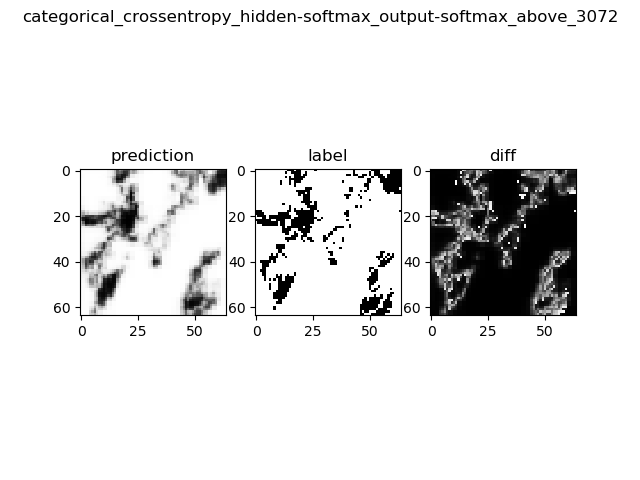
\includegraphics[width=\linewidth]{pics/categorical_crossentropy_hidden-softmax_output-softmax_above_3072}
\caption{Hidden layer activation: Softmax}
\label{fig:hiddenActivationSoftmax}
\end{subfigure}%
\begin{subfigure}{0.5\textwidth}
\centering
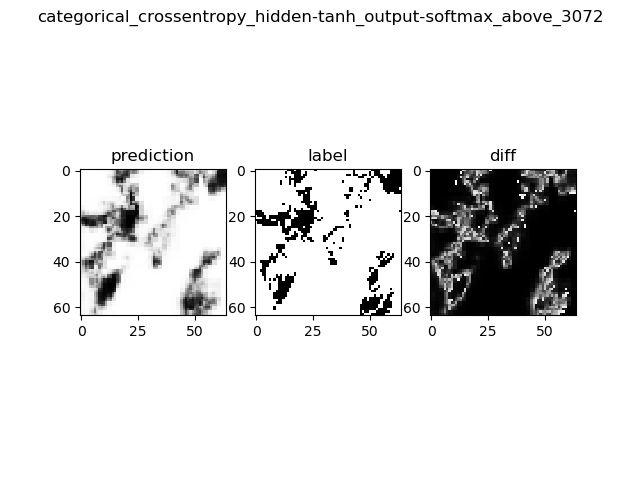
\includegraphics[width=\linewidth]{pics/categorical_crossentropy_hidden-tanh_output-softmax_above_3072}
\caption{Hidden layer activation: Tanh}
\label{fig:hiddenActivationTanh}
\end{subfigure}%
\caption{Vergleich von Aktivierungsfunktionen der Hidden-Layer}
\label{fig:activatinHidden}
\end{figure}

\subsection{Herausforderungen in diesem Kapitel}
\begin{itemize}
\item Richtige Kategorien finden
\item Training mit richtiger Aktivierungsfunktion / Optimizer
\end{itemize}


% Ziel und Test: MSE

% Fazit / Ausblick

\newpage
\listoffigures
\listoftables

\bibliography{paper/bib/report.bib}
\bibliographystyle{alpha}

\end{document}
